\section{Sensoren}
\frame{
	\frametitle{Sensoren} \pause
	\vspace{5mm}
	\begin{itemize}
		\item Physikalisch:
		\begin{itemize} 
			\item GPS
			\vspace{2mm}
			\item Accelerometer/Beschleunigung
			\vspace{2mm}
			\item Helligkeit
			\vspace{2mm}
			\item Mikrofon	
		\end{itemize}
		\vspace{3mm}
		\item Virtuell:
		\begin{itemize} 
			\item Schrittzähler
			\vspace{2mm}
			\item Lineare Beschleunigung
			\vspace{2mm}
			\item Lage/Rotation
		\end{itemize}
	\end{itemize}
}

\begin{frame}[c,fragile]
	\frametitle{GPS}
	\vspace{-3mm}
	\begin{lstlisting}[language=Java]
		LocationListener listener;
		listener = new LocationListener() {
		    public void onLocationChanged(Location loc){
		    	// fetch the weather using the provided
		    	// location
		        fetchWeather(loc.getLatitude(),
		            loc.getLongitude()); 
		    }

		    public void onStatusChanged(...) {...}
		    public void onProviderEnabled(...) {...}
		    public void onProviderDisabled(...) {...}
		};
    \end{lstlisting}	
	
\end{frame}

\begin{frame}[c,fragile]
	\frametitle{GPS}
	\begin{lstlisting}[language=Java]
		// get a location manager
		LocationManager locationManager =
		    (LocationManager) getSystemService(
		        LOCATION_SERVICE);

		// request a single location update
		locationManager.requestSingleUpdate(
		    LocationManager.GPS_PROVIDER, listener,
		        getMainLooper());
		// getMainLooper() used for executing the
		// callback (ignore for now)
    \end{lstlisting}
\end{frame}

\begin{frame}[c,fragile]
	\frametitle{GPS}
	\begin{lstlisting}[language=Java]
		// request continuous location updates each
		// hour with a minimum distance of 1 km 
		locationManager.requestLocationUpdates(
		    LocationManager.GPS_PROVIDER,
		        1 * 60 * 60 * 1000, 1000, listener);
    \end{lstlisting}
    \pause
	\begin{lstlisting}[language=Java]
		// just get the last known location
		Location location = locationManager.
		    getLastKnownLocation(
		        LocationManager.PASSIVE_PROVIDER);
    \end{lstlisting}    
\end{frame}

\begin{frame}[c]
	\frametitle{Darf ich das?}
	\pause
	\begin{center}
		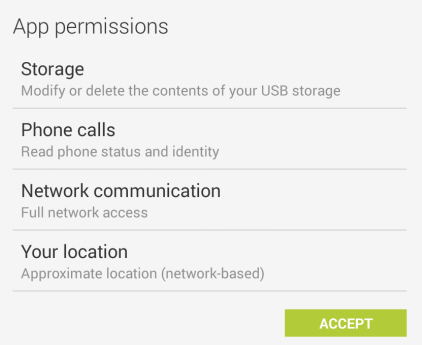
\includegraphics[width=8cm]{pictures/permissions.png}
	\end{center}
\end{frame}

\begin{frame}[c,fragile]
	\frametitle{Ja!}
	\begin{lstlisting}[language=XML]
		<uses-permission android:name=
		    "android.permission.ACCESS_FINE_LOCATION" />
		<uses-permission android:name=
		    "android.permission.ACCESS_NETWORK_STATE" />
		<uses-permission android:name=
		    "android.permission.INTERNET" />
	\end{lstlisting}
\end{frame}





